\documentclass[12pt]{article}
\usepackage[latin1]{inputenc}
% UK hyphenation
\usepackage[british]{babel}
% Copyable pdf
\usepackage{cmap}
% Font
\usepackage{lmodern}

\usepackage{amssymb, amsmath, amsthm}
\usepackage[a4paper,top=25mm,bottom=25mm,left=25mm,right=25mm]{geometry}
%\usepackage{etex}
\usepackage{ragged2e}

\usepackage{authblk} % for headings
\usepackage{pifont}
\usepackage{graphicx}
\usepackage[usenames,dvipsnames,svgnames,table]{xcolor}
\usepackage[figuresright]{rotating}
\usepackage{xtab} % tackle the long tables
\usepackage{longtable} % tackle the long tables
\usepackage{multirow}
\usepackage{footnote}
\usepackage[stable]{footmisc}
\usepackage{chngpage} % allows for temporary adjustment of side margins
\usepackage{pdflscape} % landscape environment
\usepackage{tocbibind} % includes everything in ToC

\usepackage{pgfplots}
\pgfplotsset{compat=1.14}
\pgfplotsset{every tick label/.append style={font=\footnotesize}}
\usepackage{setspace}
%\doublespacing

\makesavenoteenv{tabular}
\usepackage{tabularx}
\usepackage{booktabs}
\usepackage{threeparttable} % [flushleft]
\usepackage[referable]{threeparttablex} % footnotes in tabu
\newcolumntype{R}{>{\raggedleft\arraybackslash}X}
\newcolumntype{L}{>{\raggedright\arraybackslash}X}
\newcolumntype{C}{>{\centering\arraybackslash}X}
\newcolumntype{A}{>{\columncolor{gray!25}}C}
\newcolumntype{a}{>{\columncolor{gray!25}}c}

% Tabulator in itemize environment 
\newlength{\tablen}
\newcommand\tabbox[2][\tablen]{\makebox[#1][l]{#2}}

\usepackage{dcolumn} % alignment to decimal points
\newcolumntype{.}{D{.}{.}{-1}}

\usepackage{tikz}
\usetikzlibrary{arrows, calc, matrix, patterns, positioning, trees}
\usepackage[semicolon]{natbib}
\usepackage[hyphens]{url}
\usepackage{hyperref} % [hidelinks]
\hypersetup{
  colorlinks   = true,    		% Colours links instead of ugly boxes
  urlcolor     = blue,    		% Colour for external hyperlinks
  linkcolor    = blue,			% Colour of internal links
  citecolor    = ForestGreen,		  	% Colour of citations
}
\usepackage{microtype}
\usepackage[justification=centering]{caption} % [justification=centering]

% Captions of subtables and subfigures
\usepackage[labelformat=simple]{subcaption}
\renewcommand\thesubfigure{\alph{subfigure}}
\DeclareCaptionLabelFormat{parenthesis}{(#2)}
\captionsetup[subfigure]{labelformat=parenthesis,font+=small,list=false}
\makeatletter
\renewcommand\p@subfigure{\arabic{figure}.}
\makeatother

\renewcommand\thesubtable{\alph{subtable}}
\DeclareCaptionLabelFormat{parenthesis}{(#2)}
\captionsetup[subtable]{labelformat=parenthesis,font+=small,list=false}
\makeatletter
\renewcommand\p@subtable{\arabic{table}.}
\makeatother

% Pgfplot common legend
\newenvironment{customlegend}[1][]{%
	\begingroup
        % inits/clears the lists (which might be populated from previous
        % axes):
	\csname pgfplots@init@cleared@structures\endcsname
	\pgfplotsset{#1}%
    }{%
	% draws the legend:
	\csname pgfplots@createlegend\endcsname
	\endgroup
    }%
    % makes \addlegendimage available (typically only available within an
    % axis environment):
\def\addlegendimage{\csname pgfplots@addlegendimage\endcsname}

\usepackage{enumitem}

% felsorolasok behuzasa
\setlist[itemize]{leftmargin=2.5\parindent}
\setlist[enumerate]{leftmargin=2.5\parindent}

\theoremstyle{plain}
\newtheorem{assumption}{Assumption}%[section]
\newtheorem{conjecture}{Conjecture}[section]
\newtheorem{corollary}{Corollary}[section]
\newtheorem{lemma}{Lemma}[section]
\newtheorem{proposition}{Proposition}[section]
\newtheorem{result}{Result}
\newtheorem{theorem}{Theorem}[section]

\theoremstyle{definition}
\newtheorem{axiom}{Axiom}[section]
\newtheorem{condition}{Condition}[section]
\newtheorem{definition}{Definition}[section]
\newtheorem{example}{Example}%[section]
\newtheorem{problem}{Problem}[section]

\theoremstyle{remark}
\newtheorem{notation}{Notation}[section]
\newtheorem{remark}{Remark}[section]

\newcommand{\aproof}{\hfill{\ding{111}}}

% Sakk elemzeshez kell
\newcommand{\down}{\textcolor{BrickRed}{\rotatebox[origin=c]{270}{\ding{212}}}}
\newcommand{\up}{\textcolor{PineGreen}{\rotatebox[origin=c]{90}{\ding{212}}}}

\def\keywords{\vspace{.5em} % Add keywords
{\noindent \textit{Keywords}: }}
\def\endkeywords{\par}

\def\AMS{\vspace{.5em} % Add keywords
{\noindent \textbf{\emph{MSC} class}: }}
\def\endAMS{\par}

\def\JEL{\vspace{.5em} % Add keywords
{\noindent \textbf{\emph{JEL} classification number}: }}
\def\endJEL{\par}

\title{Improving the fairness of constrained assignments: The role of draw order in the UEFA Champions League}
\author{\href{https://sites.google.com/view/laszlocsato}{L\'aszl\'o Csat\'o}\thanks{~E-mail: \emph{laszlo.csato@sztaki.hu}} }
\affil{Institute for Computer Science and Control (SZTAKI) \\
E\"otv\"os Lor\'and Research Network (ELKH) \\
Laboratory on Engineering and Management Intelligence \\
Research Group of Operations Research and Decision Systems}
\affil{Corvinus University of Budapest (BCE) \\
Institute of Operations and Decision Sciences \\
Department of Operations Research and Actuarial Sciences}
\affil{Budapest, Hungary}
\date{\today}

\def\Dedication{
{\noindent
``\emph{Overall, we show that, although marginally better randomizations \emph{are} possible, the tournament's transparency-first procedure under our objective resembles the fairest possible lottery over the constrained assignments.}''\footnote{~Source: \citet[p.~2]{BoczonWilson2022}.}
}}
\def\endDedication{\par}

\begin{document}

\newgeometry{top=15mm,bottom=15mm,left=25mm,right=25mm}
\maketitle
\thispagestyle{empty}
\Dedication

\begin{abstract}
\noindent
The organiser of the UEFA Champions League, one of the most prestigious football tournaments in the world, faces a non-trivial mechanism design problem each autumn: how to choose a perfect matching in a balanced bipartite graph randomly. For the sake of credibility and transparency, the Round of 16 draw consists of some discrete uniform choices from two urns whose compositions are dynamically updated with computer assistance. Even though the adopted mechanism is unevenly distributed over all valid assignments, it resembles the fairest possible lottery according to a recent result. We challenge this finding by analysing the effect of reversing the order of the urns. The optimal draw procedure is shown to be primarily dependent on the lexicographic order of degree sequences for the two sets of teams. An example is provided where exchanging the urns can reduce unfairness by one-third on average and almost halve the worst bias for all pairs of teams. Nonetheless, the current policy of starting the draw with the runners-up remains the best option if the draw order should be determined before the national associations of the clubs are known.
\end{abstract}
% Since the set of edges depends on the national associations of the teams playing in the Round of 16, the graph is almost guaranteed to change in every season.

\keywords{constrained assignment; draw mechanism; fairness; tournament design; UEFA Champions League}

\AMS{90-10, 91B14, 90B90}
% Mathematical modeling or simulation for problems pertaining to operations research and mathematical programming
% Social Choice
% Case-oriented studies in operations research

\JEL{C44, C63, Z20}
% Operations Research, Statistical Decision Theory
% Computational Techniques, Simulation Modeling 
% Sports Economics, General

\clearpage
\restoregeometry

\section{Introduction} \label{Sec1}

In many allocation problems, randomisation is a crucial goal of the designer because any non-random assignment is often regarded as unfair \citep{BudishCheKojimaMilgrom2013}. However, the existence of a perfect randomisation procedure does not guarantee that it will be accepted by the stakeholders, especially if the randomisation is implemented by an obscure computer code. Consequently, the allocation mechanism should also be perceived and understood as fair by all participants, which usually implies that it needs to allow the verification of each calculation at least ex-post. 

The Union of European Football Associations (UEFA) faces a similar challenge each autumn. In particular, the UEFA Champions League---one of the most prestigious football tournaments in the world and the most prestigious club competition in European football---involves a complex assignment problem in its Round of 16 draw: to select a perfect matching in a balanced bipartite graph.
In order to ensure ex-ante \emph{fairness}, all valid assignments should occur with the same probability. This can be easily achieved by listing all feasible outcomes and drawing one of them randomly.
However, UEFA does not use this procedure because of at least two reasons.
First, it would be boring to watch, which is important since the draw ceremony is streamed live over the internet and broadcast by several media companies \citep{BoczonWilson2022}.
Second, it would be impossible to detect fraud and prevent conspiracy theories---but checking credibility is a crucial aspect since the ex-post outcome will certainly favour some teams at the expense of others.

Therefore, UEFA has adopted an easy to follow randomisation procedure. At the beginning of the draw, the names of the clubs are physically placed in two urns. The draw consists of discrete uniform choices from the urns and can be observed by the public. The composition of the urns is dynamically updated with computer assistance to ensure that all constraints will be satisfied. Even though the computer-assisted algorithm is essentially a black box and carries out non-trivial calculations, all computations are deterministic and can be verified during or after the draw with basic mathematical knowledge. For instance, a mistake was detected in the draw of the 2021/22 season, hence, the whole process was repeated three hours later \citep{Guyon2021d}.

Naturally, there is no ``free lunch'' and the randomisation mechanism chosen by UEFA is unfair, i.e., the feasible outcomes are not equally likely \citep{Kiesl2013, KlossnerBecker2013}. Nonetheless, utilising the main result of \citet{BudishCheKojimaMilgrom2013}, \citet{BoczonWilson2022} have recently demonstrated that the design of the UEFA Champions League Round of 16 draw is near-optimal and close to a constrained-best solution as it resembles the fairest possible lottery over the constrained assignments.

We refine and, to some degree, challenge this important finding of \citet{BoczonWilson2022} by analysing the effect of reversing the role of the two urns in the UEFA Champions League Round of 16 draw.
Our main contributions can be summarised as follows:
\begin{itemize}
\item
The optimal draw procedure is shown to be primarily dependent on the lexicographic order of degree sequences for the two sets of teams (group winners and runners-up) (Sections~\ref{Sec41} and \ref{Sec42});
\item
An example is provided where exchanging the urns is able to reduce the unfairness of the randomisation procedure by one-third on average and almost halve the worst bias for all pairs of teams (Section~\ref{Sec43});
\item
Unfairness is presented to be a non-monotonic function of exclusions, that is, adding a new restriction can bring the mechanism closer to the ideal evenly distributed draw (Section~\ref{Sec44});
\item
The current UEFA policy of starting the draw with the runners-up is documented and explained to be the better option if the draw order should be determined in advance, before the national associations of the clubs are known (Sections~\ref{Sec41} and \ref{Sec42}).
\end{itemize}
Most of these findings are unexpected. Even though the potential impact of the draw order has been recognised \citep[Proposition~2]{BoczonWilson2022}, it has been called slight \citep[Footnote~19]{KlossnerBecker2013} and minimal for the 2017/18 \citep{Guyon2017b}, 2019/20 \citep{Guyon2019d}, and 2022/23 seasons \citep{Guyon2022c} by a leading expert of the field.\footnote{~The French mathematician \emph{Julien Guyon} proposed a reform of the FIFA World Cup draw in the \emph{New York Times} \citep{Guyon2014b} and \emph{Le Monde} \citep{Guyon2014d} in June 1014. One of his recommendations---that is essentially equivalent to the procedure used in the UEFA Champions League Round of 16 draw \citep{Csato2023g}---has been adopted for both the 2018 \citep{Guyon2018d} and 2022 \citep{Csato2023d} FIFA World Cups, which is among the greatest achievements of academic research in the design of sports rules.}
In addition, since several scenarios exist where the more favourable order of the urns decreases the level of unfairness by at least 20\%, the statement of \citet[p.~9]{BoczonWilson2022} that ``\emph{the gain from a fairness-optimal randomization is marginal}'' appears to be a rough simplification of the issue.
%Consequently, the current study offers a novel example of how operations research and applied mathematics can contribute to the design of sports tournaments \cite{Wright2014, Csato2021a}.

%The paper is organised as follows.
%Section~\ref{Sec2} describes the rules of the UEFA Champions League Round of 16 draw. The research problem and the methodology are introduced in Section~\ref{Sec3}, while the main contributions are presented in Section~\ref{Sec4}. Section~\ref{Sec5} summarises our findings and raises open questions.

\section{The UEFA Champions League Round of 16 draw} \label{Sec2}

The UEFA Champions League is contested by the best European football clubs that can qualify primarily based on the results of their domestic leagues in the previous year. Since the 1997/98 season, multiple entrants are allowed from certain countries; now the strongest leagues can provide up to five teams as has happened for Germany in 2022/23.

The Champions League is organised in the same format since the 2003/04 season: a group stage played in eight home-away round-robin groups, where the top two teams qualify for the knockout stage starting from the Round of 16.
%The knockout phase consists of two-legged clashes, each team plays one game home and one away, except for the final, which is played in a predetermined neutral field. 
% There are no draw restrictions in later rounds of the knockout stage, each team can meet all the others.
In the Round of 16, the eight group winners and the eight runners-up need to be divided into eight mutually disjoint pairs subject to the following restrictions:
\begin{itemize}
\item
\emph{Bipartite constraint}: a group winner is not allowed to play against a runner-up;
\item
\emph{Group constraint}: teams from the same group cannot be paired;
\item
\emph{Association constraint}: teams from the same country cannot be matched.
\end{itemize}
On 17 July 2014, the UEFA emergency panel decided that Ukrainian and Russian clubs could not be drawn against each other ``until further notice'' due to political reasons. This rule has been effective only in the 2015/16 season and can be treated similarly to the association constraint by considering Russia and Ukraine as the same country.

The first restriction, the bipartite constraint, reduces the number of valid assignments to $8! = 40320$ as every result of the draw can be represented by a permutation of the eight groups.
The second restriction, the group constraint, means that only a derangement (a permutation without a fixed point, in other words, a permutation where no element appears in its original position) is allowed, which decreases the number of feasible solutions to 14833 \citep{KlossnerBecker2013}.
The impact of the association constraint depends on the identity of the teams. Thus, no simple combinatorial formula exists to determine the number of possible results of the draw. For instance, there have been 4781 feasible assignments in the 2020/21 season \citep{Guyon2021c} but only 3876 in the 2022/2023 season \citep{Guyon2022c}.
%Even though the restrictions substantially reduce the number of possible matchings, there are still thousands of them.

The Round of 16 draw is equivalent to selecting a perfect matching in a balanced bipartite graph with $2 \times 8$ nodes.
UEFA uses the following mechanism for this purpose:
\begin{itemize}
\item
Eight balls containing the names of the eight runners-up are placed in a bowl;
\item
A ball is drawn from the bowl, and the team drawn plays at home in match 1;
\item
The computer shows which group winners are eligible to play as the visiting team in match 1;
\item
Balls representing these teams are placed in another bowl;
\item
A ball is drawn from the second bowl to complete the pairing for match 1;
\item
The above procedure is repeated for the remaining matches.
\end{itemize}
The computer may indicate that only one group winner is allowed to play as the visiting team when this team is automatically assigned to the match.

The mechanism is more complicated than it seems at first glance because it should be checked not only whether draw conditions apply for the runner-up chosen at the moment, but also whether draw conditions are anticipated to apply for the runner(s)-up still to be drawn. Let us see the following illustration.

\begin{table}[t!]
  \centering
  \caption{Teams playing in the 2012/13 UEFA Champions League Round of 16}
  \label{Table1}
    \rowcolors{1}{gray!20}{}
    \begin{tabularx}{0.9\textwidth}{cLlLl} \toprule \hiderowcolors
    \multirow{2}[0]{*}{Group} & \multicolumn{2}{c}{Runner-up} & \multicolumn{2}{c}{Group winner} \\
          & Club  & Country & Club  & Country \\ \bottomrule \showrowcolors
    A     & Porto & Portugal & Paris Saint-Germain & France \\
    B     & Arsenal & England & Schalke 04 & Germany \\
    C     & Milan & Italy & M\'alaga & Spain \\
    D     & Real Madrid & Spain & Borussia Dortmund & Germany \\
    E     & Shakhtar Donetsk & Ukraine & Juventus & Italy \\
    F     & Valencia & Spain & Bayern M\"unchen & Germany \\
    G     & Celtic Glasgow & Scotland & Barcelona & Spain \\
    H     & Galatasaray & Turkey & Manchester United & England \\ \bottomrule
    \end{tabularx}
\end{table}

\begin{example} \label{Examp1} \citep{KlossnerBecker2013}
The participants of the 2012/13 UEFA Champions League Round of 16 are shown in Table~\ref{Table1}.
The draw happened as follows:
\begin{enumerate}
\item
The runner-up Galatasaray was drawn first. Its eligible opponents were all teams except for Manchester United owing to the group constraint. Out of the seven group winners, Schalke 04 was drawn.
\item
The runner-up Celtic Glasgow was drawn second. Its possible opponents were all teams except for Schalke 04 (already drawn), and Barcelona (group constraint). Out of the six group winners, Juventus was drawn.
\item
The runner-up Arsenal was drawn third. Its admissible opponents were all teams except for Schalke 04, Juventus (already drawn), and Manchester United (association constraint). The group constraint was ineffective. Out of the five group winners, Bayern M\"unchen was drawn.
\item
The runner-up Shakhtar Donetsk was drawn fourth. Its eligible opponents were all teams except for Schalke 04, Juventus, and Bayern M\"unchen (already drawn). Out of the five remaining group winners, Borussia Dortmund was drawn.
\item
The runner-up Milan was drawn fifth. The computer indicated that it should be paired with Barcelona, hence, no draw was carried out.
\end{enumerate}
Does this indicate a flaw? Naturally not. Four group winners (Paris Saint-Germain, M\'alaga, Barcelona, Manchester United) remained to be drawn. M\'alaga was prohibited by the group constraint. If Milan would have played against the French or English team, then three pairings would have been left with four Spanish clubs (Real Madrid, Valencia, M\'alaga, Barcelona), and the association constraint would have been violated.

However, two (Real Madrid, Valencia) out of the three remaining runners-up still could have faced either Paris Saint-Germain or Manchester United. Therefore, the draw was not finished in the fifth round after Milan was drawn.
\end{example}

In the following, the procedure above will be called the \emph{standard UEFA mechanism}.

This procedure always leads to a valid matching if there is an assignment satisfying all constraints. The existence can be proved by Hall's marriage theorem analogously to \citet{Kiesl2013}, but now the maximal number of teams in the Round of 16 is five for at most two countries. The result appears in \citet[Chapter~3.6]{Haigh2019} as an application of mathematics in everyday life.

The same algorithm is used in other UEFA club tournaments such as the UEFA Europa League and the UEFA Europa Conference League for the draw of the knockout round play-offs and the Round of 16 \citep{Csato2022d}.
Furthermore, it is applied to allocate teams into groups with more than two teams in several competitions for national teams \citep{Csato2023g}: the FIBA Basketball World Cup, the UEFA Euro qualifying, the UEFA Nations League, and the European Qualifiers to the FIFA World Cup. After a reform inspired by the criticism of \citet{Guyon2015a}, the FIFA World Cup draw is also carried out by this randomisation mechanism since 2018 \citep{Guyon2018d, Csato2023d}.

\section{Research question and methodology} \label{Sec3}

The (standard) UEFA mechanism is distinct from a uniform draw over all admissible matchings \citep{BoczonWilson2022, Guyon2014a, Kiesl2013, KlossnerBecker2013}. Even though the distortions in pairwise match probabilities seem to be small, it is relatively frequent that a certain club $i$ plays against club $j$ with a higher probability than against club $k$ according to an evenly distributed draw, but a match between $i$ and $k$ has a higher chance to occur than a match between $i$ and $j$ according to the UEFA mechanism \citep{KlossnerBecker2013}. In addition, even the small probability differences may change the expected revenue of some teams by more than 10 thousand euros due to the substantial amount of prize money \citep{KlossnerBecker2013}.
%These oddities would still be present if at every point during the procedure, a random choice would be made whether to match a winner to a runner-up or vice versa \citep[Footnote~19]{KlossnerBecker2013}.

Hence, the expected outcome needs to be as close to the fair uniform draw as possible.
\citet{BoczonWilson2022} examine all possible counterfactual lotteries over the feasible assignments to conclude that the current draw mechanism is near-optimal. Nonetheless, it is worth analysing whether the \emph{reversed UEFA mechanism}, where the group winners are drawn first instead of the runners-up, is able to yield a fairer outcome than the standard version.  

As an illustration, let us see the implied probabilities for the 2012/13 UEFA Champions League Round of 16 draw.

\begin{example} \label{Examp2}
Consider the three draw procedures (uniform choice among all valid assignments, standard UEFA mechanism, reversed UEFA mechanism) in Example~\ref{Examp1} with the teams listed in Table~\ref{Table1}.

\begin{table}[t!]
  \centering
  \caption{Probabilities for each pair of teams in the 2012/13 \\ UEFA Champions League Round of 16, uniform draw}
  \label{Table2}
    \rowcolors{1}{gray!20}{}
\centerline{
    \begin{tabularx}{1.1\textwidth}{l CCCCCCCC} \toprule \hiderowcolors
    \multirow{2}[0]{*}{Runner-up} & \multicolumn{8}{c}{Group of the group winner} \\
          & A     & B     & C     & D     & E     & F     & G     & H \\ \bottomrule \showrowcolors
    Porto & 0     & 11.64\% & 18.96\% & 12.37\% & 13.34\% & 12.37\% & 18.25\% & 13.05\% \\
    Arsenal & 13.05\% & 0     & 22.22\% & 14.17\% & 15.14\% & 14.17\% & 21.25\% & 0 \\
    Milan & 14.48\% & 14.68\% & 0     & 15.54\% & 0     & 15.54\% & 23.19\% & 16.57\% \\
    Real Madrid & 18.40\% & 18.78\% & 0     & 0     & 21.76\% & 19.55\% & 0 & 21.51\% \\
    Shakhtar Donetsk & 11.68\% & 11.83\% & 19.31\% & 12.61\% & 0     & 12.61\% & 18.71\% & 13.25\% \\
    Valencia & 18.40\% & 18.78\% & 0     & 19.55\% & 21.76\% & 0     & 0     & 21.51\% \\
    Celtic Glasgow & 12.36\% & 12.52\% & 20.14\% & 13.20\% & 14.48\% & 13.20\% & 0     & 14.11\% \\
    Galatasaray & 11.64\% & 11.77\% & 19.37\% & 12.56\% & 13.51\% & 12.56\% & 18.60\% & 0 \\ \bottomrule
    \end{tabularx}
}
\end{table}

Table~\ref{Table2} presents the ideal probabilities according to an evenly distributed draw.
The association constraint is effective for six pairs: Arsenal and Manchester United (winner of Group H), Milan and Juventus (winner of Group E), Real Madrid and M\'alaga (winner of Group C), Real Madrid and Barcelona (winner of Group G), Valencia and M\'alaga, Valencia and Barcelona.
There are 5463 valid matchings; among them, Porto plays against Schalke 04 (winner of Group B) in 636 cases, against M\'alaga in 1036 cases, and so on.
Note that the probabilities of Porto vs Borussia Dortmund (winner of Group D) and Porto vs Bayern M\"unchen (winner of Group F) coincide ($676/5463 \approx 12.37\%$) because the two German group winners are symmetric as the runners-up in their groups are Spanish teams. On the other hand, the probabilities for Schalke 04 are different because the runner-up in its group is the English club Arsenal.
Analogously, the matches Porto vs Manchester United and Arsenal vs Paris Saint-Germain (winner of Group A) have the same probability of $731/5463 \approx 13.05\%$ as both Porto and Paris-Saint Germain come from Group A without an association constraint, while both Arsenal and Manchester United are English clubs such that the other team from their groups (Schalke 04 and Galatasaray, respectively) is without an association constraint, and there are no more English teams. These numbers have already appeared in \citet[Tabelle~2]{Kiesl2013} and \citet[Table~4]{KlossnerBecker2013}.

\begin{table}[t!]
  \centering
  \caption{Probabilities for each pair of teams in the 2012/13 \\ UEFA Champions League Round of 16, standard draw mechanism}
  \label{Table3}
    \rowcolors{1}{gray!20}{}
\centerline{
    \begin{tabularx}{1.1\textwidth}{l CCCCCCCC} \toprule \hiderowcolors
    \multirow{2}[0]{*}{Runner-up} & \multicolumn{8}{c}{Group of the group winner} \\
          & A     & B     & C     & D     & E     & F     & G     & H \\ \bottomrule \showrowcolors
    Porto & 0     & 11.70\% & 18.85\% & 12.21\% & 13.44\% & 12.21\% & 18.30\% & 13.30\% \\
    Arsenal & 13.38\% & 0     & 21.68\% & 14.21\% & 15.54\% & 14.20\% & 21.00\% & 0 \\
    Milan & 14.38\% & 14.63\% & 0     & 15.47\% & 0     & 15.47\% & 23.46\% & 16.59\% \\
    Real Madrid & 18.34\% & 18.71\% & 0     & 0     & 21.57\% & 20.14\% & 0     & 21.25\% \\
    Shakhtar Donetsk & 11.70\% & 11.90\% & 19.38\% & 12.43\% & 0     & 12.42\% & 18.63\% & 13.53\% \\
    Valencia & 18.36\% & 18.69\% & 0     & 20.14\% & 21.57\% & 0     & 0     & 21.25\% \\
    Celtic Glasgow & 12.16\% & 12.36\% & 20.89\% & 13.13\% & 14.23\% & 13.14\% & 0     & 14.08\% \\
    Galatasaray & 11.68\% & 12.02\% & 19.21\% & 12.41\% & 13.65\% & 12.42\% & 18.62\% & 0 \\ \bottomrule
    \end{tabularx}
}
\end{table}

Table~\ref{Table3} shows the probabilities according to the standard UEFA mechanism, approximated by 50 million simulated draws. A similar technique has been used by \citet{BoczonWilson2022}, too, as can be seen in \citet[Table~1]{BoczonWilson2022}.
The greatest bias occurs for the pair Celtic Glasgow vs M\'alaga, which exceeds 0.75 percentage points.
These numbers have already appeared in \citet[Tabelle~3]{Kiesl2013} and \citet[Table~5]{KlossnerBecker2013}; the small differences are due to the inaccuracy of our simulations.

\begin{table}[t!]
  \centering
  \caption{Probabilities for each pair of teams in the 2012/13 \\ UEFA Champions League Round of 16, reversed draw mechanism}
  \label{Table4}
    \rowcolors{1}{gray!20}{}
\centerline{
    \begin{tabularx}{1.1\textwidth}{l CCCCCCCC} \toprule \hiderowcolors
    \multirow{2}[0]{*}{Runner-up} & \multicolumn{8}{c}{Group of the group winner} \\
          & A     & B     & C     & D     & E     & F     & G     & H \\ \bottomrule \showrowcolors
    Porto & 0     & 11.68\% & 18.88\% & 12.16\% & 13.50\% & 12.16\% & 18.25\% & 13.38\% \\
    Arsenal & 13.30\% & 0     & 21.88\% & 14.10\% & 15.54\% & 14.09\% & 21.08\% & 0 \\
    Milan & 14.37\% & 14.60\% & 0     & 15.49\% & 0     & 15.47\% & 23.47\% & 16.60\% \\
    Real Madrid & 18.37\% & 18.69\% & 0     & 0     & 21.46\% & 20.36\% & 0     & 21.12\% \\
    Shakhtar Donetsk & 11.71\% & 11.90\% & 19.35\% & 12.39\% & 0     & 12.40\% & 18.62\% & 13.62\% \\
    Valencia & 18.36\% & 18.70\% & 0     & 20.37\% & 21.47\% & 0     & 0     & 21.10\% \\
    Celtic Glasgow & 12.20\% & 12.41\% & 20.65\% & 13.13\% & 14.31\% & 13.13\% & 0     & 14.18\% \\
    Galatasaray & 11.69\% & 12.02\% & 19.23\% & 12.37\% & 13.72\% & 12.38\% & 18.58\% & 0 \\ \bottomrule
    \end{tabularx}
}
\end{table}

Finally, Table~\ref{Table4} contains the (simulated) probabilities according to the reversed UEFA mechanism.
The greatest bias occurs for the pair Valencia vs Borussia Dortmund, which exceeds 0.81 percentage points.
These numbers have not appeared before in the literature, although the expected result of the reversed randomisation procedure has already been presented for the 2017/18 \citep{Guyon2017b}, 2019/20 \citep{Guyon2019d}, and 2022/23 seasons \citep{Guyon2022c}, based on one million simulation runs.
\end{example}

The fairness of the standard and reversed UEFA mechanisms will be evaluated by focusing on the probability of matches played in the Round of 16. Let $p_{ij}$ be the ideal probability that clubs $i$ and $j$ are matched under the evenly distributed uniform draw, and $p_{ij}^M$ be the probability of this event if mechanism $M$ is used to obtain a feasible assignment. Two fairness distortion measures for mechanism $M$ are defined as follows:
\begin{equation} \label{eq_AFD}
\mathit{AFD}(M) = 1000 \times \frac{\sum_{i,j} \left| p_{ij} - p_{ij}^M \right|}{\sum_{i,j} \# \left\{ p_{ij} > 0 \right\}},
\end{equation}
\begin{equation} \label{eq_MFD}
\mathit{MFD}(M) = 100 \times \max_{i,j} \left| p_{ij} - p_{ij}^M \right|,
\end{equation}
where $\sum_{i,j} \# \left\{ p_{ij} > 0 \right\}$ is the number of team pairs with a positive probability. Its maximum is 56 if the association constraint is ineffective, but this has never happened in the UEFA Champions League since 2003; the denominator varies between 43 (2019/20) and 53 (five seasons). The multipliers of thousand and hundred in formulas~\eqref{eq_AFD} and \eqref{eq_MFD}, respectively, are normalising factors.

$\mathit{AFD}$ is called \emph{average fairness distortion} and $\mathit{MFD}$ is called \emph{maximal fairness distortion}. The crucial difference between them is that $\mathit{AFD}$ allows the draw mechanism to compensate for the increased unfairness in a particular team pair with a reduction in other team pairs, while this is not possible under $\mathit{MFD}$. Furthermore, the value of $\mathit{MFD}$ has a more straightforward interpretation: how much is the probability of a potential match in the Round of 16 changed by mechanism $M$ compared to the uniform draw \emph{in the worst case}.

\citet{BoczonWilson2022} use a more complicated quantification of fairness, which computes the average absolute difference in the match likelihoods across all valid pairwise comparisons. However, their distortion metric equals zero only if there are no constraints in the draw, and increases with the number of restricted team pairs. On the other hand, both $\mathit{AFD}$ and $\mathit{MFD}$ are zero for the perfect uniform draw among all feasible matchings.

In the comparison of two draw procedures $M1$ and $M2$, the number of team pairs for which one of them provides a less biased probability than the other, can also be interesting. This inspires our pair fairness measure:
\begin{equation} \label{eq_PF}
\mathit{PF}(M1, M2) = 2 \times \frac{\sum_{i,j} \# \left\{ \left| p_{ij} - p_{ij}^{M1} \right| < \left| p_{ij} - p_{ij}^{M2} \right| \right\}}{\sum_{i,j} \# \left\{ \left| p_{ij} - p_{ij}^{M1} \right| \neq \left| p_{ij} - p_{ij}^{M2} \right| \right\}} -1.
\end{equation}
Consequently, $\mathit{PF}(M1, M2)$ is between $-1$ and $+1$ such that it equals $-1$ if mechanism $M2$ implies a less distorted probability than mechanism $M1$ for all team pairs, while $+1$ indicates the complete dominance of $M1$ over $M2$.

\section{Results} \label{Sec4}

Section~\ref{Sec41} studies the fairness of the standard and reversed UEFA mechanisms based on historical data. Some findings from this investigation will be elaborated in Sections~\ref{Sec42}--\ref{Sec44}.

\subsection{Historical UEFA Champions League seasons} \label{Sec41}

\begin{table}[t!]
  \centering
  \caption{Associations with more than one team \\ in the UEFA Champions League Round of 16}
  \label{Table5}
\centerline{
\begin{threeparttable}
    \rowcolors{1}{gray!20}{}
    \begin{tabularx}{1.2\textwidth}{r CCC CCC CCC CCC CCC CCC} \toprule \hiderowcolors
    \multirow{2}[0]{*}{Season} & \multicolumn{3}{c}{England} & \multicolumn{3}{c}{France} & \multicolumn{3}{c}{Germany} & \multicolumn{3}{c}{Italy} & \multicolumn{3}{c}{Portugal} & \multicolumn{3}{c}{Spain} \\
          & 1    & 2    & $\Delta$  & 1    & 2    & $\Delta$  & 1    & 2    & $\Delta$  & 1    & 2    & $\Delta$  & 1    & 2    & $\Delta$  & 1    & 2    & $\Delta$ \\  \bottomrule \showrowcolors
    2003/04 & 3     & 0     & 3     & 2     & 0     & 2     & 0     & 2     & $-$2    & 2     & 0     & 2     & 0     & 1     & $-$1    & 1     & 3     & $-$2 \\
    2004/05 & 2     & 2     & 0     & 2     & 0     & 2     & 1     & 2     & $-$1    & 3     & 0     & 3     & 0     & 1     & $-$1    & 0     & 2     & $-$2 \\
    2005/06 & 2     & 1     & 1     & 1     & 0     & 1     & 0     & 2     & $-$2    & 3     & 0     & 3     & 0     & 1     & $-$1    & 2     & 1     & 1 \\
    2006/07 & 4     & 0     & 4     & 1     & 1     & 0     & 1     & 0     & 1     & 1     & 2     & $-$1    & 0     & 1     & $-$1    & 1     & 2     & $-$1 \\
    2007/08 & 2     & 2     & 0     & 0     & 1     & $-$1    & 0     & 1     & $-$1    & 2     & 1     & 1     & 1     & 0     & 1     & 3     & 0     & 3 \\
    2008/09 & 2     & 2     & 0     & 0     & 1     & $-$1    & 1     & 0     & 1     & 2     & 1     & 1     & 1     & 1     & 0     & 1     & 3     & $-$2 \\
    2009/10 & 3     & 0     & 3     & 1     & 1     & 0     & 0     & 2     & $-$2    & 1     & 2     & $-$1    & 0     & 1     & $-$1    & 3     & 0     & 3 \\
    2010/11 & 3     & 1     & 2     & 0     & 2     & $-$2    & 2     & 0     & 2     & 0     & 3     & $-$3    & 0     & 0     & 0     & 2     & 1     & 1 \\
    2011/12 & 2     & 0     & 2     & 0     & 2     & $-$2    & 1     & 1     & 0     & 1     & 2     & $-$1    & 1     & 0     & 1     & 2     & 0     & 2 \\
    2012/13 & 1     & 1     & 0     & 1     & 0     & 1     & 3     & 0     & 3     & 1     & 1     & 0     & 0     & 1     & $-$1    & 2     & 2     & 0 \\
    2013/14 & 2     & 2     & 0     & 1     & 0     & 1     & 2     & 2     & 0     & 0     & 1     & $-$1    & 0     & 0     & 0     & 3     & 0     & 3 \\
    2014/15 & 1     & 2     & $-$1    & 1     & 1     & 0     & 2     & 2     & 0     & 0     & 1     & $-$1    & 1     & 0     & 1     & 3     & 0     & 3 \\
    2015/16 & 2     & 1     & 1     & 0     & 1     & $-$1    & 2     & 0     & 2     & 0     & 2     & $-$2    & 0     & 1     & $-$1    & 3     & 0     & 3 \\
    2016/17 & 2     & 1     & 1     & 1     & 1     & 0     & 1     & 2     & $-$1    & 2     & 0     & 2     & 0     & 2     & $-$2    & 2     & 2     & 0 \\
    2017/18 & 4     & 1     & 3     & 1     & 0     & 1     & 0     & 1     & $-$1    & 1     & 1     & 0     & 0     & 1     & $-$1    & 1     & 2     & $-$1 \\
    2018/19 & 1     & 3     & $-$2    & 1     & 1     & 0     & 2     & 1     & 1     & 1     & 1     & 0     & 1     & 0     & 1     & 2     & 1     & 1 \\
    2019/20 & 2     & 2     & 0     & 1     & 1     & 0     & 2     & 1     & 1     & 1     & 2     & $-$1    & 0     & 0     & 0     & 2     & 2     & 0 \\
    2020/21 & 3     & 0     & 3     & 1     & 0     & 1     & 2     & 2     & 0     & 1     & 2     & $-$1    & 0     & 1     & $-$1    & 1     & 3     & $-$2 \\
    2021/22 & 3     & 1     & 2     & 1     & 1     & 0     & 1     & 0     & 1     & 1     & 1     & 0     & 0     & 2     & $-$2    & 1     & 2     & $-$1 \\
    2022/23 & 3     & 1     & 2     & 0     & 1     & $-$1    & 1     & 3     & $-$2    & 1     & 2     & $-$1    & 2     & 0     & 2     & 1     & 0     & 1 \\ \bottomrule
    Average & \multicolumn{3}{c}{1.2} & \multicolumn{3}{c}{0.05} & \multicolumn{3}{c}{0} & \multicolumn{3}{c}{$-$0.05} & \multicolumn{3}{c}{$-$0.35} & \multicolumn{3}{c}{0.5} \\ \toprule
	\end{tabularx}
\begin{tablenotes} \footnotesize
\item
\emph{Notes}: Column 1 shows the number of group winners; Column 2 shows the number of runners-up; Column $\Delta$ shows the difference between the number of group winners and runners-up.
\item
The last row shows the average of Column $\Delta$ for each country.
\item
The number of exclusions for any national association equals the number of group winners times the number of runners-up. The only exception is the season 2005/06 when Chelsea and Liverpool both qualified from Group G---thus, the number of constraints due to England is one rather than two. In addition, a Russian group winner could not have played against a Ukrainian runner-up in 2015/16.
\end{tablenotes}
\end{threeparttable}
}
\end{table}

Between 2003/04 and 2022/23, 20 seasons have been played in the UEFA Champions League according to the same rules with respect to the Round of 16 draw. Six countries have had more than one club qualified for the Round of 16 in at least one year as can be seen in Table~\ref{Table5}, which also gives some information on the number of exclusions due to the association constraint. For instance, the one group winner and the three runners-up from Spain have implied three prohibited clashes in 2003/04.

\begin{figure}[t!]
\centering

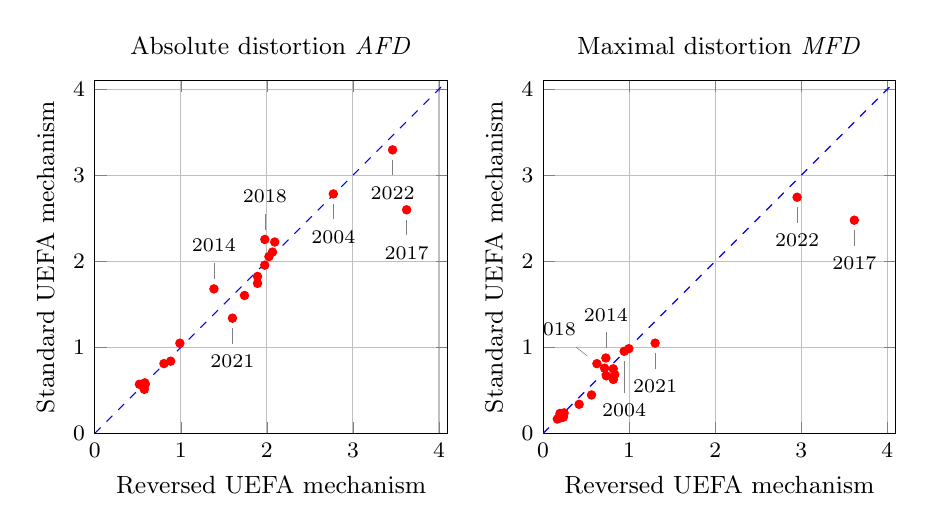
\begin{tikzpicture}
\begin{axis}[
name = axis1,
title = {Absolute distortion $\mathit{AFD}$},
title style = {font=\small},
xlabel = Reversed UEFA mechanism,
x label style = {font=\small},
ylabel = Standard UEFA mechanism,
y label style = {font=\small},
width = 0.5\textwidth,
height = 0.5\textwidth,
nodes near coords,
xmajorgrids = true,
ymajorgrids = true,
xmin = 0,
xmax = 4.1,
ymin = 0,
ymax = 4.1,
]
\addplot [scatter,red,only marks,mark size=1.5pt,point meta=explicit symbolic] coordinates {
(0.989599020898075,1.04832279448298)
(2.77272162609176,2.78287689950249)
(0.882225922887611,0.839184282198522)
(0.804479536247259,0.811377006231495)
(1.89173619290457,1.82378600478088)
(2.09160762935801,2.22406950934172)
(0.587055198243915,0.571544174180777)
(1.74005987458943,1.60285124713845)
(0.519550231666842,0.57101108560184)
(1.89160499769357,1.74399211861615)
(0.581640971308739,0.587354304642073)
(1.38512771352651,1.67930541674952)
(0.576116745979197,0.512016244278464)
(1.97576352798896,1.95554048557555)
(3.62429179262455,2.59846861187892)
(1.97642062090336,2.2538359400523)
(2.06549367098018,2.10715692679413)
(2.0241129339814,2.05515532494286)
(1.60021187831083,1.33937602567988)
(3.46137598899209,3.29469615239078)
};
% Zero line
\draw [blue,dashed] (rel axis cs:0,0) -- (rel axis cs:1,1);
% Graph
\node[pin={[pin distance=0.2cm, ultra thick] 270:{\textcolor{black}{\scriptsize{2004}}}}] at (2.77272162609176,2.78287689950249) {};
\node[pin={[pin distance=0.2cm, ultra thick] 90:{\textcolor{black}{\scriptsize{2014}}}}] at (1.38512771352651,1.67930541674952) {};
\node[pin={[pin distance=0.2cm, ultra thick] 270:{\textcolor{black}{\scriptsize{2017}}}}] at (3.62429179262455,2.59846861187892) {};
\node[pin={[pin distance=0.2cm, ultra thick] 90:{\textcolor{black}{\scriptsize{2018}}}}] at (1.97642062090336,2.2538359400523) {};
\node[pin={[pin distance=0.2cm, ultra thick] 270:{\textcolor{black}{\scriptsize{2021}}}}] at (1.60021187831083,1.33937602567988) {};
\node[pin={[pin distance=0.2cm, ultra thick] 270:{\textcolor{black}{\scriptsize{2022}}}}] at (3.46137598899209,3.29469615239078) {};
\end{axis}

\begin{axis}[
at = {(axis1.south east)},
xshift = 0.1\textwidth,
title = {Maximal distortion $\mathit{MFD}$},
title style = {font=\small},
xlabel = Reversed UEFA mechanism,
x label style = {font=\small},
ylabel = Standard UEFA mechanism,
y label style = {font=\small},
width = 0.5\textwidth,
height = 0.5\textwidth,
nodes near coords,
xmajorgrids = true,
ymajorgrids = true,
xmin = 0,
xmax = 4.1,
ymin = 0,
ymax = 4.1,
]
\addplot [scatter,red,only marks,mark size=1.5pt,point meta=explicit symbolic] coordinates {
(0.166188033034451,0.167207834827748)
(0.942906657084946,0.954354657084946)
(0.419310695652172,0.338294695652175)
(0.244454213373402,0.238726213373402)
(0.816824827546955,0.627172827546957)
(0.99677626773762,0.984714267737619)
(0.207653831977128,0.181931603254895)
(0.563012893401013,0.446758893401017)
(0.196529376626217,0.232209376626216)
(0.815580031850632,0.750775291231923)
(0.187393291392624,0.184253291392622)
(0.729732062001773,0.876386062001772)
(0.236607376626216,0.189567961080137)
(0.735236570694087,0.669658224507283)
(3.61684049551675,2.47753449551675)
(0.625820781808339,0.810602740660529)
(0.714800317682318,0.758046317682318)
(0.83265158850227,0.684134974281392)
(1.30230718510772,1.04947518510772)
(2.95202711455108,2.74443511455108)
};
% Zero line
\draw [blue,dashed] (rel axis cs:0,0) -- (rel axis cs:1,1);
% Graph
\node[pin={[pin distance=0.4cm, ultra thick] 270:{\textcolor{black}{\scriptsize{2004}}}}] at (0.942906657084946,0.954354657084946) {};
\node[pin={[pin distance=0.2cm, ultra thick] 90:{\textcolor{black}{\scriptsize{2014}}}}] at (0.729732062001773,0.876386062001772) {};
\node[pin={[pin distance=0.2cm, ultra thick] 270:{\textcolor{black}{\scriptsize{2017}}}}] at (3.61684049551675,2.47753449551675) {};
\node[pin={[pin distance=0.1cm, ultra thick] 120:{\textcolor{black}{\scriptsize{2018}}}}] at (0.625820781808339,0.810602740660529) {};
\node[pin={[pin distance=0.2cm, ultra thick] 270:{\textcolor{black}{\scriptsize{2021}}}}] at (1.30230718510772,1.04947518510772) {};
\node[pin={[pin distance=0.2cm, ultra thick] 270:{\textcolor{black}{\scriptsize{2022}}}}] at (2.95202711455108,2.74443511455108) {};
\end{axis}
\end{tikzpicture}

\caption{Fairness distortions of the draw mechanisms \\ in the UEFA Champions League Round of 16 \\ \vspace{0.2cm}
\footnotesize{\emph{Note}: Seasons are denoted by their first year (e.g.\ 2022 stands for 2022/23) since the Round of 16 draw takes place each autumn. Our notation is different from \citet{BoczonWilson2022}, who use the second year.}}
\label{Fig1}

\end{figure}

Figure~\ref{Fig1} compares the standard and reversed UEFA mechanisms by the two measures of fairness distortion. Each dot represents one of the 20 seasons; a dot below (above) the dashed 45-degree line implies that the standard (reversed) procedure is fairer. As expected, the order of the urns cannot fundamentally improve fairness. However, the difference between the two mechanisms is non-negligible in certain seasons such as 2014/15 and 2017/18. For example, the probability of a match between Bayern M\"unchen and Liverpool in 2022/23 was reduced from the ideal 39.86\% to 37.12\% (standard) or to 36.91\% (reversed) by the randomisation procedure used.
Metrics $\mathit{AFD}$ and $\mathit{MFD}$ are similar, they usually imply the same choice between the standard and reversed versions. On the other hand, maximal fairness distortion exhibits a greater variance. According to $\mathit{MFD}$, the draw mechanism has been outstandingly unfair in seasons 2017/18 and 2022/23. The role of the draw order is somewhat increased if the randomisation procedure is less fair.

\begin{figure}[t!]
\centering

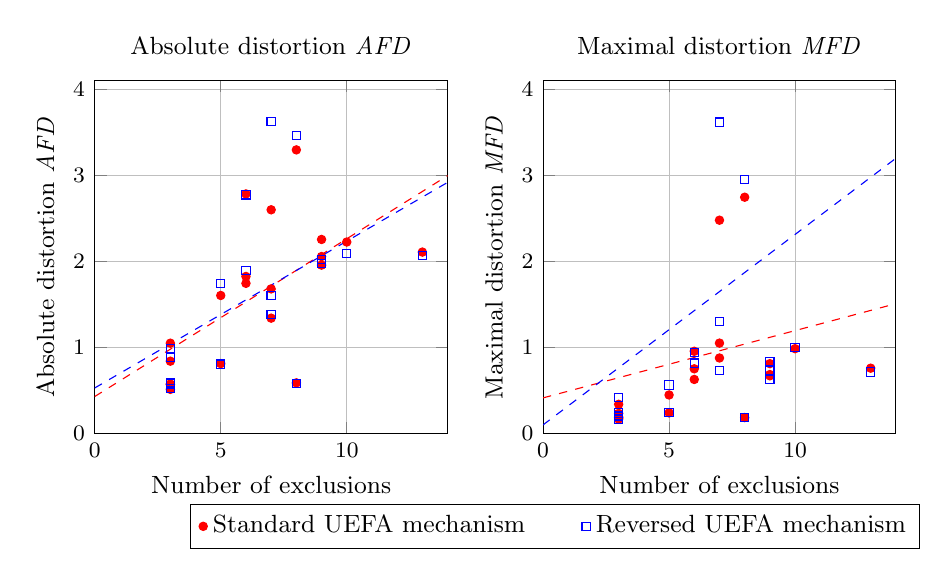
\begin{tikzpicture}
\begin{axis}[
name = axis1,
title = {Absolute distortion $\mathit{AFD}$},
title style = {font=\small},
xlabel = Number of exclusions,
x label style = {font=\small},
ylabel = Absolute distortion $\mathit{AFD}$,
y label style = {font=\small},
width = 0.5\textwidth,
height = 0.5\textwidth,
nodes near coords,
xmajorgrids = true,
ymajorgrids = true,
xmin = 0,
xmax = 14,
ymin = 0,
ymax = 4.1,
]
% Standard
\addplot [scatter,red,only marks,mark size=1.5pt,point meta=explicit symbolic] coordinates {
(3,1.04832279448298)
(6,2.78287689950249)
(3,0.839184282198522)
(5,0.811377006231495)
(6,1.82378600478088)
(10,2.22406950934172)
(3,0.571544174180777)
(5,1.60285124713845)
(3,0.57101108560184)
(6,1.74399211861615)
(8,0.587354304642073)
(7,1.67930541674952)
(3,0.512016244278464)
(9,1.95554048557555)
(7,2.59846861187892)
(9,2.2538359400523)
(13,2.10715692679413)
(9,2.05515532494286)
(7,1.33937602567988)
(8,3.29469615239078)
};
% Trend line
\draw[red,dashed] (\pgfkeysvalueof{/pgfplots/xmin},0.1833 * \pgfkeysvalueof{/pgfplots/xmin} + 0.4286) -- (\pgfkeysvalueof{/pgfplots/xmax},0.1833 * \pgfkeysvalueof{/pgfplots/xmax} + 0.4286);

% Reversed
\addplot [scatter,blue,only marks,mark=square,mark size=1.5pt,point meta=explicit symbolic] coordinates {
(3,0.989599020898075)
(6,2.77272162609176)
(3,0.882225922887611)
(5,0.804479536247259)
(6,1.89173619290457)
(10,2.09160762935801)
(3,0.587055198243915)
(5,1.74005987458943)
(3,0.519550231666842)
(6,1.89160499769357)
(8,0.581640971308739)
(7,1.38512771352651)
(3,0.576116745979197)
(9,1.97576352798896)
(7,3.62429179262455)
(9,1.97642062090336)
(13,2.06549367098018)
(9,2.0241129339814)
(7,1.60021187831083)
(8,3.46137598899209)
};
% Trend line
\draw[blue,dashed] (\pgfkeysvalueof{/pgfplots/xmin},0.176 * \pgfkeysvalueof{/pgfplots/xmin} + 0.528) -- (\pgfkeysvalueof{/pgfplots/xmax},0.176 * \pgfkeysvalueof{/pgfplots/xmax} + 0.4528);
\end{axis}

\begin{axis}[
at = {(axis1.south east)},
xshift = 0.1\textwidth,
title = {Maximal distortion $\mathit{MFD}$},
title style = {font=\small},label = Reversed UEFA mechanism,
xlabel = Number of exclusions,
x label style = {font=\small},
ylabel = Maximal distortion $\mathit{MFD}$,
y label style = {font=\small},
width = 0.5\textwidth,
height = 0.5\textwidth,
nodes near coords,
xmajorgrids = true,
ymajorgrids = true,
xmin = 0,
xmax = 14,
ymin = 0,
ymax = 4.1,
legend style = {font=\small,at={(-1,-0.2)},anchor=north west,legend columns=2},
legend entries = {Standard UEFA mechanism$\qquad$,Reversed UEFA mechanism},
]
% Standard
\addplot [scatter,red,only marks,mark size=1.5pt,point meta=explicit symbolic] coordinates {
(3,0.167207834827748)
(6,0.954354657084946)
(3,0.338294695652175)
(5,0.238726213373402)
(6,0.627172827546957)
(10,0.984714267737619)
(3,0.181931603254895)
(5,0.446758893401017)
(3,0.232209376626216)
(6,0.750775291231923)
(8,0.184253291392622)
(7,0.876386062001772)
(3,0.189567961080137)
(9,0.669658224507283)
(7,2.47753449551675)
(9,0.810602740660529)
(13,0.758046317682318)
(9,0.684134974281392)
(7,1.04947518510772)
(8,2.74443511455108)
};
% Trend line
\draw[red,dashed] (\pgfkeysvalueof{/pgfplots/xmin},0.0986 * \pgfkeysvalueof{/pgfplots/xmin} + 0.41271) -- (\pgfkeysvalueof{/pgfplots/xmax},0.0986 * \pgfkeysvalueof{/pgfplots/xmax} + 0.1271);

% Reversed
\addplot [scatter,blue,only marks,mark=square,mark size=1.5pt,point meta=explicit symbolic] coordinates {
(3,0.166188033034451)
(6,0.942906657084946)
(3,0.419310695652172)
(5,0.244454213373402)
(6,0.816824827546955)
(10,0.99677626773762)
(3,0.207653831977128)
(5,0.563012893401013)
(3,0.196529376626217)
(6,0.815580031850632)
(8,0.187393291392624)
(7,0.729732062001773)
(3,0.236607376626216)
(9,0.735236570694087)
(7,3.61684049551675)
(9,0.625820781808339)
(13,0.714800317682318)
(9,0.83265158850227)
(7,1.30230718510772)
(8,2.95202711455108)
};
% Trend line
\draw[blue,dashed] (\pgfkeysvalueof{/pgfplots/xmin},0.2213 * \pgfkeysvalueof{/pgfplots/xmin} + 0.099) -- (\pgfkeysvalueof{/pgfplots/xmax},0.2213 * \pgfkeysvalueof{/pgfplots/xmax} + 0.099);
\end{axis}
\end{tikzpicture}

\caption{Fairness distortions of the draw mechanisms in the UEFA \\ Champions League Round of 16 by the number of association constraints \\ \vspace{0.2cm}
\footnotesize{\emph{Note}: Dashed lines indicate fitted linear relationship.}}
\label{Fig2}

\end{figure}

Figure~\ref{Fig2} shows how unfairness depends on the number of prohibited clashes by the association constraint. As the dashed linear trends reveal, the bias of the draw mechanism tends to be greater if there are more constraints, but the relationship is rather weak. For instance, although there were eight country restrictions in both the 2013/14 and the 2022/23 seasons, the draw of the former was among the fairest, and the draw of the latter was among the least fair. Contrarily, the fairness distortions were about the same in the three seasons (2016/17, 2018/19, 2020/21) with nine exclusions.

\begin{table}[t!]
  \centering
  \caption{Summary of the historical UEFA Champions League Round of 16 draws}
  \label{Table6}
\centerline{
\begin{threeparttable}
    \rowcolors{1}{}{gray!20}
    \begin{tabularx}{1.15\textwidth}{l ccRRRRrc} \toprule \hiderowcolors   
    \multirow{3}[0]{*}{Season} & Number of & Number of & \multicolumn{4}{c}{Change in fairness distortion} & \multicolumn{1}{c}{Pair}  & Degree \\
          & valid & exclusions & \multicolumn{2}{c}{Absolute} & \multicolumn{2}{c}{Relative} & \multicolumn{1}{c}{fairness} & sequence \\
          & solutions &       & $\mathit{AFD}$   & $\mathit{MFD}$   & $\mathit{AFD}$   & $\mathit{MFD}$   & \multicolumn{1}{c}{$\mathit{PF}$} & order \\ \bottomrule \showrowcolors
    2003/04 & 8476  & 3     & $-$0.059 & $-$0.001 & $-$5.60\% & $-$0.61\% & $-$0.321 & $-$1 \\
    2004/05 & 5427  & 6     & $-$0.010 & $-$0.011 & $-$0.36\% & $-$1.20\% & $-$0.080 & $-$1 \\
    2005/06 & 9200  & 3     & 0.043 & 0.081 & 5.13\% & 23.95\% & 0.094 & 1 \\
    2006/07 & 6655  & 5     & $-$0.007 & 0.006 & $-$0.85\% & 2.40\% & 0.020 & $-$1 \\
    2007/08 & 5271  & 6     & 0.068 & 0.190 & 3.73\% & 30.24\% & 0.120 & 1 \\
    2008/09 & 2988  & 10    & $-$0.132 & 0.012 & $-$5.96\% & 1.22\% & $-$0.261 & $-$1 \\
    2009/10 & 9094  & 3     & 0.016 & 0.026 & 2.71\% & 14.14\% & 0.170 & $-$1 \\
    2010/11 & 6304  & 5     & 0.137 & 0.116 & 8.56\% & 26.02\% & 0.216 & 1 \\
    2011/12 & 9147  & 3     & $-$0.051 & $-$0.036 & $-$9.01\% & $-$15.37\% & $-$0.208 & $-$1 \\
    2012/13 & 5463  & 6     & 0.148 & 0.065 & 8.46\% & 8.63\% & 0.280 & 0 \\
    2013/14 & 3497  & 8     & $-$0.006 & 0.003 & $-$0.97\% & 1.70\% & 0.042 & 0 \\
    2014/15 & 4516  & 7     & $-$0.294 & $-$0.147 & $-$17.52\% & $-$16.73\% & $-$0.633 & $-$1 \\
    2015/16 & 9147  & 3     & 0.064 & 0.047 & 12.52\% & 24.81\% & 0.208 & 1 \\
    2016/17 & 3501  & 9     & 0.020 & 0.066 & 1.03\% & 9.79\% & 0.021 & 0 \\
    2017/18 & 4238  & 7     & 1.026 & 1.139 & 39.48\% & 45.99\% & 0.429 & 1 \\
    2018/19 & 3694  & 9     & $-$0.277 & $-$0.185 & $-$12.31\% & $-$22.80\% & $-$0.617 & $-$1 \\
    2019/20 & 2002  & 13    & $-$0.042 & $-$0.043 & $-$1.98\% & $-$5.70\% & $-$0.349 & 0 \\
    2020/21 & 3305  & 9     & $-$0.031 & 0.149 & $-$1.51\% & 21.71\% & $-$0.149 & $-$1 \\
    2021/22 & 4781  & 7     & 0.261 & 0.253 & 19.47\% & 24.09\% & 0.551 & 1 \\
    2022/23 & 3876  & 8     & 0.167 & 0.208 & 5.06\% & 7.56\% & 0.125 & -1 \\ \bottomrule
    Average & 5529  & 6.5   & 0.052 & 0.097 & 2.50\% & 8.99\% & $-$0.017 & $-$0.2 \\ \toprule
    Optimal & ---   & ---   & $-$0.045 & $-$0.021 & $-$2.80\% & $-$3.12\% & \multicolumn{1}{c}{---} & --- \\ \bottomrule
    \end{tabularx}
\begin{tablenotes} \footnotesize
\item
\emph{Note}: The column Degree sequence order compares lexicographically the degree sequences of the group winners and the runners-up. $-$1 indicates that the degree sequence of the group winners is greater; 0 indicates that the two degree sequences are equal; $+$1 indicates that the degree sequence of the runners-up is greater.
\end{tablenotes}
\end{threeparttable}
}
\end{table}

Exchanging the two bowls would have been the most advantageous in the 2018/19 season according to Table~\ref{Table6}. The table also uncovers that the reversed draw order ensured a better outcome with an improvement of at least 5\% in 5 (4) from the last 20 seasons according to average (maximal) fairness distortion. However, the choice of UEFA was analogously justified in 7 (11) seasons by the metric $\mathit{AFD}$ ($\mathit{MFD}$). Consequently, the bias of the draw would have been increased by 2.5\% (9\%) on average if the group winners would have been drawn first. Adopting the optimal draw order before the event is expected to reduce the level of unfairness by about 3\%. Even though this improvement is not so powerful at first sight, it is still worth considering since the reform is convenient and even a small step towards fairness is welcomed if it has such a small price.

Reassuringly, the pair fairness metric $\mathit{PF}$ shows a similar picture to $\mathit{AFD}$ and $\mathit{MFD}$. For instance, in the 2014/15 season, the standard UEFA mechanism implies a fairer probability for nine pairs out of 49, but the reversed version is fairer in the remaining 40 cases. The standard procedure is better for 12 years and the reversed variant is optimal in eight years, although the difference is almost negligible in certain seasons such as 2006/07.

Finally, note that both the standard and the reversed UEFA randomisation procedure should be fairer than its pair with the same chance from a purely mathematical point of view: if the sets of group winners and runners-up are exchanged, then the optimal order of the bowls will be reversed, too. Hence, the reversed UEFA mechanism has the potential to improve fairness by more than 28\% based on the 2017/18 Champions League season. However, this nice symmetry does not hold in the real-world if the clubs from some national associations are more likely to win their groups than being runners-up or vice versa---for which Table~\ref{Table5} gives solid evidence.

\begin{result} \label{Res1}
The mechanism of the UEFA Champions League Round of 16 draw would have been fairer by reversing the order of two urns in some seasons. The benefit of this change can be quite robust, and it seems to be worth exploiting due to the low implementation costs.
However, if the draw order should be chosen before the national associations of the participating clubs are known, then the current policy is optimal.
\end{result}

\subsection{Balanced bipartite graphs with eight nodes} \label{Sec42}

Figure~\ref{Fig2} does not reveal the underlying reason of the difference between the standard and reversed draw mechanisms. Unfortunately, it is difficult to get more insight into this issue in the setting of the Champions League Round of 16 draw owing to the high number of possible exclusions and their arrangement in the corresponding bipartite graph. Hence, we have simplified the problem to a potential draw for the quarterfinals with four group winners and four runners-up where both the association and group constraints apply. In that case, complete enumeration is within reach, but the results are far from trivial.

\input{Figure3_n=4_all_unfair_graphs}

Figure~\ref{Fig3} presents all balanced bipartite graphs with eight nodes where a feasible solution exists and the UEFA randomisation procedure is biased. For example, in graph $G_3$ (Figure~\ref{Fig3c}), team $D$ (the winner of the only group that is not affected by association constraints) has $1/3 = 48/144$ chance to play against team $a$ under the uniform draw, but this probability is $2/7 = 40/144$ under the standard and $43/144$ under the reversed UEFA mechanism.

\input{Figure4_n=4_fairness_distortion}

Figure~\ref{Fig4} presents the fairness distortions for these six graphs. The values of $\mathit{AFD}$ are by an order of magnitude higher compared to the historical Champions League seasons because the constraints more severely restrict the set of solutions due to the low number of nodes. On the other hand, maximal distortion does still not exceed 7\%, showing that the UEFA randomisation procedure is not fundamentally flawed. The two measures rank the graphs differently with respect to fairness: while the standard mechanism performs the best for $G_1$ according to $\mathit{AFD}$, it becomes the worst for this graph according to $\mathit{MFD}$.

Even though the UEFA mechanism is biased for six bipartite graphs, there is no difference between its standard and reversed variants for four symmetric graphs ($G_1$, $G_2$, $G_4$, $G_6$) where the two sets of nodes can be exchanged. This condition does not hold for $G_3$ and $G_5$, which have different degree sequences for the group winners and the runners-up. In both cases, the reversed draw mechanism is closer to fairness and the degree sequence of the group winners is lexicographically greater than the degree sequence of the runners-up, meaning that the association constraint is more ``concentrated'' for the group winners as there are more runners-up than group winners from an association.

Therefore, the lexicographical order of the two degree sequences is entirely responsible for the difference between the standard and reversed UEFA mechanisms in the reduced-dimensional problem with eight nodes. The functional relationship does not hold for bipartite graphs with 16 nodes, but the association remains quite strong according to the last three columns of Table~\ref{Table6}. In particular, there is only one season (2022/23) where the improvement by changing the draw order is non-negligible by both $\mathit{AFD}$ and $\mathit{MFD}$, but contrary to the lexicographical order of the two degree sequences. In addition, the reversed draw procedure would have been less fair than the standard in the 2012/13 seasons, even though the degree sequences coincide.

The degree sequences of the group winners and runners-up are determined by the associations from which at least two teams qualify for the Round of 16. According to Table~\ref{Table5}, these countries are usually overrepresented among the group winners compared to the runners-up, mainly due to the strong performance of English and, to a smaller extent, Spanish clubs in the group stage. This might explain the advantage of the standard UEFA mechanism on the basis of past seasons that has been found in Section~\ref{Sec41}. 

\begin{result} \label{Res2}
In the reduced assignment problem with eight nodes, the optimal order of the two urns is fully determined by the lexicographical order of the degree sequences for the two sets of nodes. Although the functional relationship does not extend to the UEFA Champions League Round of 16 draw, it remains highly likely that the standard UEFA mechanism is not worse than its reversed variant if the degree sequence of the group winners is greater. This finding provides a partial explanation for the superiority of the standard draw procedure on the basis of historical data.
\end{result}

\subsection{Case study 1: graphs with a fixed degree sequence} \label{Sec43}

As Section~\ref{Sec42} uncovered, the lexicographical order of degree sequences for the group winners and runners-up has a substantial impact on the relative performance of the standard and reversed UEFA mechanisms. In order to study further this relationship, eight bipartite graphs have been chosen with the same degree sequence, where all clubs have the same number of constraints---but their arrangements are different. 

\input{Figure5_n=8_3211_selected_graphs}

Figure~\ref{Fig5} shows these graphs, each of them having seven exclusions such that no runner-up is affected by more than one association constraint, while a group winner is affected by three, and another by two such restrictions. The group constraints apply as before. The number of valid solutions depends on the structure of constraints only to a small extent.

\input{Figure6_n=8_3211_fairness_distortion}

However, the level of unfairness is strongly influenced by the arrangement of the restrictions as presented in Figure~\ref{Fig6}: for example, the fairness distortion of the standard draw mechanism is increased by more than 80\% (170\%) in graph $H_5$ compared to $H_7$ according to the metric $\mathit{AFD}$ ($\mathit{MFD}$). Because of the fixed degree sequence, the reversed procedure is less biased than the standard version for all these graphs. On the other hand, the degree of improvement varies between 3.5\% (graph $H_5$, average fairness distortion) and almost 50\% (graph $H_1$, maximal fairness distortion). The advantage of the reversed mechanism is always higher according to the measure $\mathit{MFD}$, but even the reduction in the average bias exceeds 33\% for graph $H_1$.

\begin{result} \label{Res3}
Even if the degree sequences are fixed, the size of fairness distortions and the relative effect of the draw order depend to a great extent on the arrangement of the constraints. There exists an example where the reversed procedure decreases the average level of unfairness by one-third, while almost halves the bias in the worst case.
\end{result}

\subsection{Case study 2: graphs with an increasing set of exclusions} \label{Sec44}

%\input{Preambulum}

\begin{figure}[t!]
\centering
\begin{subfigure}{0.24\textwidth}
\centering
\caption{$I_1$: \#12714}
\label{Fig7a}

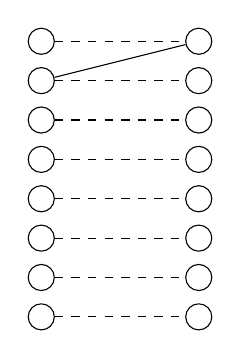
\begin{tikzpicture}[scale=1, auto=center]
\tikzstyle{every node}=[draw,shape=circle];
  \node[minimum size=0.25cm] (n1) at (0,3.5) {};
  \node[minimum size=0.25cm] (n2) at (0,3)   {};
  \node[minimum size=0.25cm] (n3) at (0,2.5) {};
  \node[minimum size=0.25cm] (n4) at (0,2)   {};
  \node[minimum size=0.25cm] (n5) at (0,1.5) {};
  \node[minimum size=0.25cm] (n6) at (0,1)   {};
  \node[minimum size=0.25cm] (n7) at (0,0.5) {};
  \node[minimum size=0.25cm] (n8) at (0,0)   {};
  \node[minimum size=0.25cm] (n9) at (2,3.5) {};
  \node[minimum size=0.25cm] (n10) at (2,3)   {};
  \node[minimum size=0.25cm] (n11) at (2,2.5) {};
  \node[minimum size=0.25cm] (n12) at (2,2)   {};
  \node[minimum size=0.25cm] (n13) at (2,1.5) {};
  \node[minimum size=0.25cm] (n14) at (2,1)   {};
  \node[minimum size=0.25cm] (n15) at (2,0.5) {};
  \node[minimum size=0.25cm] (n16) at (2,0)   {};

  \foreach \from/\to in {n1/n9,n2/n10,n3/n11,n4/n12,n5/n13,n6/n14,n7/n15,n8/n16}
    \draw[dashed] (\from) -- (\to);
  \foreach \from/\to in {n2/n9}
    \draw (\from) -- (\to);
\end{tikzpicture}
\end{subfigure}
\begin{subfigure}{0.24\textwidth}
\centering
\caption{$I_2$: \#10904}
\label{Fig7b}

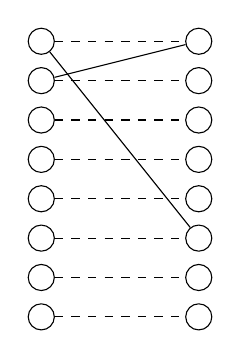
\begin{tikzpicture}[scale=1, auto=center]
\tikzstyle{every node}=[draw,shape=circle];
  \node[minimum size=0.25cm] (n1) at (0,3.5) {};
  \node[minimum size=0.25cm] (n2) at (0,3)   {};
  \node[minimum size=0.25cm] (n3) at (0,2.5) {};
  \node[minimum size=0.25cm] (n4) at (0,2)   {};
  \node[minimum size=0.25cm] (n5) at (0,1.5) {};
  \node[minimum size=0.25cm] (n6) at (0,1)   {};
  \node[minimum size=0.25cm] (n7) at (0,0.5) {};
  \node[minimum size=0.25cm] (n8) at (0,0)   {};
  \node[minimum size=0.25cm] (n9) at (2,3.5) {};
  \node[minimum size=0.25cm] (n10) at (2,3)   {};
  \node[minimum size=0.25cm] (n11) at (2,2.5) {};
  \node[minimum size=0.25cm] (n12) at (2,2)   {};
  \node[minimum size=0.25cm] (n13) at (2,1.5) {};
  \node[minimum size=0.25cm] (n14) at (2,1)   {};
  \node[minimum size=0.25cm] (n15) at (2,0.5) {};
  \node[minimum size=0.25cm] (n16) at (2,0)   {};

  \foreach \from/\to in {n1/n9,n2/n10,n3/n11,n4/n12,n5/n13,n6/n14,n7/n15,n8/n16}
    \draw[dashed] (\from) -- (\to);
  \foreach \from/\to in {n1/n14,n2/n9}
    \draw (\from) -- (\to);
\end{tikzpicture}
\end{subfigure}
\begin{subfigure}{0.24\textwidth}
\centering
\caption{$I_3$: \#9094}
\label{Fig7c}

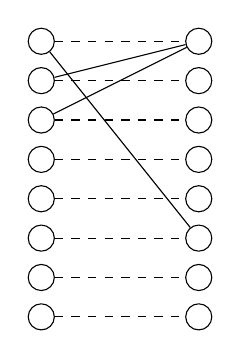
\begin{tikzpicture}[scale=1, auto=center]
\tikzstyle{every node}=[draw,shape=circle];
  \node[minimum size=0.25cm] (n1) at (0,3.5) {};
  \node[minimum size=0.25cm] (n2) at (0,3)   {};
  \node[minimum size=0.25cm] (n3) at (0,2.5) {};
  \node[minimum size=0.25cm] (n4) at (0,2)   {};
  \node[minimum size=0.25cm] (n5) at (0,1.5) {};
  \node[minimum size=0.25cm] (n6) at (0,1)   {};
  \node[minimum size=0.25cm] (n7) at (0,0.5) {};
  \node[minimum size=0.25cm] (n8) at (0,0)   {};
  \node[minimum size=0.25cm] (n9) at (2,3.5) {};
  \node[minimum size=0.25cm] (n10) at (2,3)   {};
  \node[minimum size=0.25cm] (n11) at (2,2.5) {};
  \node[minimum size=0.25cm] (n12) at (2,2)   {};
  \node[minimum size=0.25cm] (n13) at (2,1.5) {};
  \node[minimum size=0.25cm] (n14) at (2,1)   {};
  \node[minimum size=0.25cm] (n15) at (2,0.5) {};
  \node[minimum size=0.25cm] (n16) at (2,0)   {};

  \foreach \from/\to in {n1/n9,n2/n10,n3/n11,n4/n12,n5/n13,n6/n14,n7/n15,n8/n16}
    \draw[dashed] (\from) -- (\to);
  \foreach \from/\to in {n1/n14,n2/n9,n3/n9}
    \draw (\from) -- (\to);
\end{tikzpicture}
\end{subfigure}
\begin{subfigure}{0.24\textwidth}
\centering
\caption{$I_4$: \#7858}
\label{Fig7d}

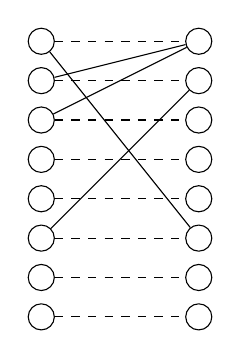
\begin{tikzpicture}[scale=1, auto=center]
\tikzstyle{every node}=[draw,shape=circle];
  \node[minimum size=0.25cm] (n1) at (0,3.5) {};
  \node[minimum size=0.25cm] (n2) at (0,3)   {};
  \node[minimum size=0.25cm] (n3) at (0,2.5) {};
  \node[minimum size=0.25cm] (n4) at (0,2)   {};
  \node[minimum size=0.25cm] (n5) at (0,1.5) {};
  \node[minimum size=0.25cm] (n6) at (0,1)   {};
  \node[minimum size=0.25cm] (n7) at (0,0.5) {};
  \node[minimum size=0.25cm] (n8) at (0,0)   {};
  \node[minimum size=0.25cm] (n9) at (2,3.5) {};
  \node[minimum size=0.25cm] (n10) at (2,3)   {};
  \node[minimum size=0.25cm] (n11) at (2,2.5) {};
  \node[minimum size=0.25cm] (n12) at (2,2)   {};
  \node[minimum size=0.25cm] (n13) at (2,1.5) {};
  \node[minimum size=0.25cm] (n14) at (2,1)   {};
  \node[minimum size=0.25cm] (n15) at (2,0.5) {};
  \node[minimum size=0.25cm] (n16) at (2,0)   {};

  \foreach \from/\to in {n1/n9,n2/n10,n3/n11,n4/n12,n5/n13,n6/n14,n7/n15,n8/n16}
    \draw[dashed] (\from) -- (\to);
  \foreach \from/\to in {n1/n14,n2/n9,n3/n9,n6/n10}
    \draw (\from) -- (\to);
\end{tikzpicture}
\end{subfigure}

\vspace{0.25cm}
\begin{subfigure}{0.24\textwidth}
\centering
\caption{$I_5$: \#6357}
\label{Fig7e}

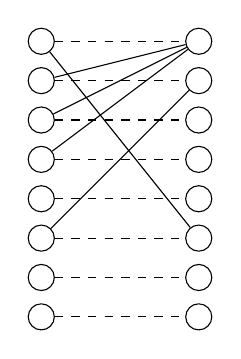
\begin{tikzpicture}[scale=1, auto=center]
\tikzstyle{every node}=[draw,shape=circle];
  \node[minimum size=0.25cm] (n1) at (0,3.5) {};
  \node[minimum size=0.25cm] (n2) at (0,3)   {};
  \node[minimum size=0.25cm] (n3) at (0,2.5) {};
  \node[minimum size=0.25cm] (n4) at (0,2)   {};
  \node[minimum size=0.25cm] (n5) at (0,1.5) {};
  \node[minimum size=0.25cm] (n6) at (0,1)   {};
  \node[minimum size=0.25cm] (n7) at (0,0.5) {};
  \node[minimum size=0.25cm] (n8) at (0,0)   {};
  \node[minimum size=0.25cm] (n9) at (2,3.5) {};
  \node[minimum size=0.25cm] (n10) at (2,3)   {};
  \node[minimum size=0.25cm] (n11) at (2,2.5) {};
  \node[minimum size=0.25cm] (n12) at (2,2)   {};
  \node[minimum size=0.25cm] (n13) at (2,1.5) {};
  \node[minimum size=0.25cm] (n14) at (2,1)   {};
  \node[minimum size=0.25cm] (n15) at (2,0.5) {};
  \node[minimum size=0.25cm] (n16) at (2,0)   {};

  \foreach \from/\to in {n1/n9,n2/n10,n3/n11,n4/n12,n5/n13,n6/n14,n7/n15,n8/n16}
    \draw[dashed] (\from) -- (\to);
  \foreach \from/\to in {n1/n14,n2/n9,n3/n9,n4/n9,n6/n10}
    \draw (\from) -- (\to);
\end{tikzpicture}
\end{subfigure}
\begin{subfigure}{0.24\textwidth}
\centering
\caption{$I_6$: \#5430}
\label{Fig7f}

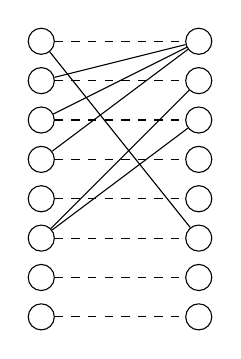
\begin{tikzpicture}[scale=1, auto=center]
\tikzstyle{every node}=[draw,shape=circle];
  \node[minimum size=0.25cm] (n1) at (0,3.5) {};
  \node[minimum size=0.25cm] (n2) at (0,3)   {};
  \node[minimum size=0.25cm] (n3) at (0,2.5) {};
  \node[minimum size=0.25cm] (n4) at (0,2)   {};
  \node[minimum size=0.25cm] (n5) at (0,1.5) {};
  \node[minimum size=0.25cm] (n6) at (0,1)   {};
  \node[minimum size=0.25cm] (n7) at (0,0.5) {};
  \node[minimum size=0.25cm] (n8) at (0,0)   {};
  \node[minimum size=0.25cm] (n9) at (2,3.5) {};
  \node[minimum size=0.25cm] (n10) at (2,3)   {};
  \node[minimum size=0.25cm] (n11) at (2,2.5) {};
  \node[minimum size=0.25cm] (n12) at (2,2)   {};
  \node[minimum size=0.25cm] (n13) at (2,1.5) {};
  \node[minimum size=0.25cm] (n14) at (2,1)   {};
  \node[minimum size=0.25cm] (n15) at (2,0.5) {};
  \node[minimum size=0.25cm] (n16) at (2,0)   {};

  \foreach \from/\to in {n1/n9,n2/n10,n3/n11,n4/n12,n5/n13,n6/n14,n7/n15,n8/n16}
    \draw[dashed] (\from) -- (\to);
  \foreach \from/\to in {n1/n14,n2/n9,n3/n9,n4/n9,n6/n10,n6/n11}
    \draw (\from) -- (\to);
\end{tikzpicture}
\end{subfigure}
\begin{subfigure}{0.24\textwidth}
\centering
\caption{$I_7$: \#4238}
\label{Fig7g}

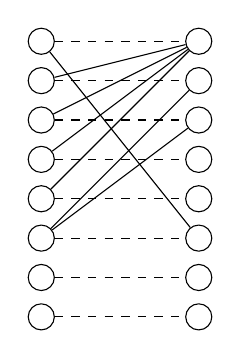
\begin{tikzpicture}[scale=1, auto=center]
\tikzstyle{every node}=[draw,shape=circle];
  \node[minimum size=0.25cm] (n1) at (0,3.5) {};
  \node[minimum size=0.25cm] (n2) at (0,3)   {};
  \node[minimum size=0.25cm] (n3) at (0,2.5) {};
  \node[minimum size=0.25cm] (n4) at (0,2)   {};
  \node[minimum size=0.25cm] (n5) at (0,1.5) {};
  \node[minimum size=0.25cm] (n6) at (0,1)   {};
  \node[minimum size=0.25cm] (n7) at (0,0.5) {};
  \node[minimum size=0.25cm] (n8) at (0,0)   {};
  \node[minimum size=0.25cm] (n9) at (2,3.5) {};
  \node[minimum size=0.25cm] (n10) at (2,3)   {};
  \node[minimum size=0.25cm] (n11) at (2,2.5) {};
  \node[minimum size=0.25cm] (n12) at (2,2)   {};
  \node[minimum size=0.25cm] (n13) at (2,1.5) {};
  \node[minimum size=0.25cm] (n14) at (2,1)   {};
  \node[minimum size=0.25cm] (n15) at (2,0.5) {};
  \node[minimum size=0.25cm] (n16) at (2,0)   {};

  \foreach \from/\to in {n1/n9,n2/n10,n3/n11,n4/n12,n5/n13,n6/n14,n7/n15,n8/n16}
    \draw[dashed] (\from) -- (\to);
  \foreach \from/\to in {n1/n14,n2/n9,n3/n9,n4/n9,n5/n9,n6/n10,n6/n11}
    \draw (\from) -- (\to);
\end{tikzpicture}
\end{subfigure}
\begin{subfigure}{0.24\textwidth}
\centering
\caption{$I_8$: \#3759}
\label{Fig7h}

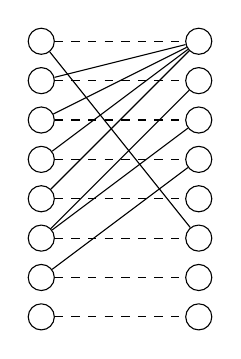
\begin{tikzpicture}[scale=1, auto=center]
\tikzstyle{every node}=[draw,shape=circle];
  \node[minimum size=0.25cm] (n1) at (0,3.5) {};
  \node[minimum size=0.25cm] (n2) at (0,3)   {};
  \node[minimum size=0.25cm] (n3) at (0,2.5) {};
  \node[minimum size=0.25cm] (n4) at (0,2)   {};
  \node[minimum size=0.25cm] (n5) at (0,1.5) {};
  \node[minimum size=0.25cm] (n6) at (0,1)   {};
  \node[minimum size=0.25cm] (n7) at (0,0.5) {};
  \node[minimum size=0.25cm] (n8) at (0,0)   {};
  \node[minimum size=0.25cm] (n9) at (2,3.5) {};
  \node[minimum size=0.25cm] (n10) at (2,3)   {};
  \node[minimum size=0.25cm] (n11) at (2,2.5) {};
  \node[minimum size=0.25cm] (n12) at (2,2)   {};
  \node[minimum size=0.25cm] (n13) at (2,1.5) {};
  \node[minimum size=0.25cm] (n14) at (2,1)   {};
  \node[minimum size=0.25cm] (n15) at (2,0.5) {};
  \node[minimum size=0.25cm] (n16) at (2,0)   {};

  \foreach \from/\to in {n1/n9,n2/n10,n3/n11,n4/n12,n5/n13,n6/n14,n7/n15,n8/n16}
    \draw[dashed] (\from) -- (\to);
  \foreach \from/\to in {n1/n14,n2/n9,n3/n9,n4/n9,n5/n9,n6/n10,n6/n11,n7/n12}
    \draw (\from) -- (\to);
\end{tikzpicture}
\end{subfigure}

\caption{Some balanced bipartite graphs with \\
16 nodes and an increasing set of exclusions \\ \vspace{0.2cm}
\footnotesize{\emph{Notes}: Dashed lines indicate the group constraints, solid lines indicate the association constraints. \\
Group winners are the nodes on the left-hand side, runners-up are the nodes on the right-hand side. \\
\# = number of valid assignments}}
\label{Fig7}
\end{figure}

%\end{document}

Finally, the impact of additional draw constraints has been investigated. The graphs considered are depicted in Figure~\ref{Fig7}. Initially, there is a single restriction owing to the national associations of the teams besides the usual group constraint (Figure~\ref{Fig7a}), however, the number of exclusions gradually increases to eight (Figure~\ref{Fig7h}). Graph $I_3$ (Figure~\ref{Fig7c}) is equivalent to the 2009/10 UEFA Champions League Round of 16 but the sets of group winners and runners-up are exchanged. Furthermore, graph $I_7$ (Figure~\ref{Fig7g}) corresponds to the 2017/18 UEFA Champions League Round of 16, where the difference between the standard and reversed draw procedures has been the highest as can be seen in Figure~\ref{Fig1}.

\input{Figure8_n=8_widening_set_fairness_distortion}

Figure~\ref{Fig8} presents the fairness distortions of the two draw mechanisms for these graphs. Even though the number of valid assignments is monotonically decreasing as a function of association restrictions, unfairness is marginally smaller when the number of exclusions grows from three to four (graphs $I_3$ and $I_4$), while it is robustly reduced by at least 20\% when the eighth constraint is added. In contrast to the result of Table~\ref{Table6}, the reversed mechanism is somewhat fairer for graph $I_3$ due to exchanging the group winners and the runners-up. However, the gain is minimal in absolute terms, and the standard draw procedure is preferred for graphs $I_5$--$I_8$.

\begin{result} \label{Res4}
Adding a new association constraint does not necessarily increase the unfairness of the UEFA Champions League Round of 16 draw.
\end{result}

\section{Conclusions} \label{Sec5}

The paper has analysed a randomisation procedure used consistently in a sports competition with high monetary stakes and serious public interest in the last 20 years. The problem of the UEFA Champions League Round of 16 draw is essentially equivalent to finding a perfect matching in a balanced bipartite graph randomly. For the sake of credibility and transparency, the draw is implemented by a specific mechanism. Although the unfairness of the draw procedure has been uncovered ten years ago \citep{Kiesl2013, KlossnerBecker2013}, it is near-optimal according to a recent paper published in a leading journal of management science \citep{BoczonWilson2022}. This result has been refined by showing that reversing the default draw order can significantly reduce the level of unfairness.

There remains a wide scope for future research. First, the reason for the difference between the standard and the reversed UEFA mechanisms has not been fully explored, although the complexity of the problem has been highlighted. Second, we have considered the effects of draw constraints only on the fairness of the draw, but they might influence the later stages of the tournament, too \citep{Csato2022d}. These issues are especially important because analogous draw conditions can be used to achieve strategic goals such as minimising the threat of unfair behaviour by the teams \citep{Csato2022a}.
Last but not least, in contrast to \citet{BoczonWilson2022}, we think tournament organisers should continue the search for fairer randomisations since all previous proposals \citep{Guyon2014a, KlossnerBecker2013, RobertsRosenthal2023} have different weaknesses.

\section*{Acknowledgements}
\addcontentsline{toc}{section}{Acknowledgements}
\noindent
This paper could not have been written without my \emph{father} (also called \emph{L\'aszl\'o Csat\'o}), who has helped to code the simulations in Python. %\\
%We are grateful to \emph{Dries Goossens}, \emph{Alex Krumer}, \emph{Frits C.~R.~Spieksma}, and \emph{Stephan Westphal} for useful advice. \\
%Five anonymous reviewers provided valuable comments and suggestions on earlier drafts. \\

\bibliographystyle{apalike}
\bibliography{All_references}

\end{document}